\documentclass[12pt]{article}
\author{Michael Schmid}
\usepackage[left=20mm,right=20mm,top=10mm,bottom=25mm]{geometry}
\usepackage[utf8]{inputenc}
\usepackage[T1]{fontenc}
\usepackage{times}
\usepackage{geometry}
\geometry{papersize={210mm,297mm},total={160mm,240mm},top=31mm,bindingoffset=15mm}
\usepackage{amsmath}
\usepackage{amssymb}
\usepackage{mathrsfs}
\usepackage{amsfonts}
\usepackage{amsthm}
\usepackage{lipsum}
\usepackage{amscd}
\usepackage{graphicx}
\usepackage{fancyhdr}
\usepackage{textcomp}
\usepackage{txfonts}
\usepackage[all]{xy}
\usepackage{paralist}
\usepackage[colorlinks=true]{hyperref}
\usepackage{array}
\usepackage{tikz}
\usepackage{slashed}
\usepackage{pdfpages}
\usepackage{cite}
\usepackage{url}
\usepackage{animate}

\usepackage{listings}
\usepackage{multirow}
\usepackage{color} %red, green, blue, yellow, cyan, magenta, black, white
\definecolor{mygreen}{RGB}{28,172,0} % color values Red, Green, Blue
\definecolor{mylilas}{RGB}{170,55,241}
\definecolor{backcolour}{rgb}{0.95,0.95,0.92}
\lstdefinestyle{Python}{
  numbers=left,
  belowcaptionskip=1\baselineskip,
  breaklines=true,
  frame=l,
  framerule=0pt,
  framesep=-1pt,
  xleftmargin=1em,
  language=Python,
  showstringspaces=false,
  basicstyle=\scriptsize\ttfamily,
  keywordstyle=\bfseries\color{green!40!black},
  commentstyle=\itshape\color{purple!40!black},
  identifierstyle=\color{blue},
  stringstyle=\color{red},
  numberstyle=\ttfamily\tiny,
  backgroundcolor=\color{backcolour}
}


\begin{document}

	\paragraph{Quadratic}

    	\begin{equation}
    	       \frac{U_{t,x}-U_{t-1,x}}{\mathrm{dt}}+\frac{U_{t,x}\,\left(U_{t,x}-U_{t,x-1}\right)}{\mathrm{dx}}=0
    	\end{equation}

        \begin{figure}[!ht]
          \centering
          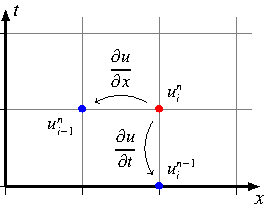
\includegraphics[width=.8\textwidth]{../tikz/quadratic/quadratic.pdf}
          \caption{Quadratic Approach Derivative}
          \label{fig:STDL}
       \end{figure}

       %
       % \begin{equation}
       %     U_{t,x} = \left(\begin{array}{c} -\frac{\mathrm{dx}-U_{x}\,\mathrm{dt}+\sqrt{{U_{x}}^2\,{\mathrm{dt}}^2-2\,U_{x}\,\mathrm{dt}\,\mathrm{dx}+4\,U_{t}\,\mathrm{dt}\,\mathrm{dx}+{\mathrm{dx}}^2}}{2\,\mathrm{dt}}\\ \frac{U_{x}\,\mathrm{dt}-\mathrm{dx}+\sqrt{{U_{x}}^2\,{\mathrm{dt}}^2-2\,U_{x}\,\mathrm{dt}\,\mathrm{dx}+4\,U_{t}\,\mathrm{dt}\,\mathrm{dx}+{\mathrm{dx}}^2}}{2\,\mathrm{dt}} \end{array}\right)
       % \end{equation}


      \begin{frame}
        \centering
        \animategraphics[loop,controls,width=\linewidth]{60}{../images/quadratic}{0}{359}
      \end{frame}

       \begin{figure}[!ht]
           \begin{minipage}[b]{0.5\textwidth}
             \includegraphics[width=1.1\textwidth]{../Quadratic_front.jpg}
             \caption{Linear Approach}
             \label{fig:STDL}
           \end{minipage}
           \begin{minipage}[b]{0.5\textwidth}
             \includegraphics[width=1\textwidth]{../Quadratic_top.jpg}
             \caption{Linear Approach}
             \label{fig:STDL}
           \end{minipage}
       \end{figure}

        \newpage
	\paragraph{Linear 1}

        \begin{equation}
            \frac{U_{t,x}-U_{t-1,x}}{\mathrm{dt}}+ U_{t,x}\, \frac{\left(U_{t-1,x}-U_{t-1,x-1}\right)}{\mathrm{dx}}=0
        \end{equation}

        \begin{figure}[!ht]
          \centering
          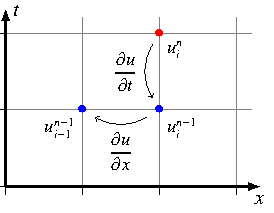
\includegraphics[width=.8\textwidth]{../tikz/linear1/linear1.pdf}
          \caption{linear Approach Derivative}
          \label{fig:STDL}
        \end{figure}

        % \begin{equation}
        %   \xi = \frac{\left(U_{t-1,x}-U_{t-1,x-1}\right)}{\mathrm{dx}}
        % \end{equation}
        %
        % \begin{equation}
        %   \frac{U_{t,x}-U_{t-1,x}}{\mathrm{dt}}+ U_{t,x}\, \xi=0
        % \end{equation}
        %
        %
        % \begin{equation}
        % U_{t,x}-U_{t-1,x}+ \mathrm{dt} \, U_{t,x}\, \xi=0
        % \end{equation}
        %
        % \begin{equation}
        % U_{t,x}+ \mathrm{dt} \, U_{t,x}\, \xi=U_{t-1,x}
        % \end{equation}
        %
        % \begin{equation}
        % U_{t,x} \left(1 + \mathrm{dt} \, \xi \right)=U_{t-1,x}
        % \end{equation}
        %
        % \begin{equation}
        % U_{t,x} = \frac{U_{t-1,x}}{1 + \mathrm{dt} \, \xi}
        % \end{equation}

        \begin{figure}[!ht]
            \begin{minipage}[b]{0.5\textwidth}
              \includegraphics[width=1.1\textwidth]{../linear1_front.jpg}
              \caption{Linear Approach}
              \label{fig:STDL}
            \end{minipage}
            \begin{minipage}[b]{0.5\textwidth}
              \includegraphics[width=1\textwidth]{../linear1_top.jpg}
              \caption{Linear Approach}
              \label{fig:STDL}
            \end{minipage}
        \end{figure}
        \newpage

    \paragraph{Linear 2}

        \begin{equation}
            \frac{U_{t,x}-U_{t-1,x}}{\mathrm{dt}}+ U_{t-1,x}\, \frac{\left(U_{t-1,x}-U_{t-1,x-1}\right)}{\mathrm{dx}}=0
        \end{equation}


        \begin{figure}[!ht]
          \centering
          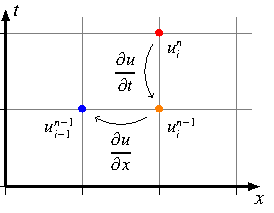
\includegraphics[width=.8\textwidth]{../tikz/linear2/linear2.pdf}
          \caption{linear Approach Derivative}
          \label{fig:STDL}
        \end{figure}

        \begin{figure}[!ht]
            \begin{minipage}[b]{0.5\textwidth}
              \includegraphics[width=1.1\textwidth]{../linear2_front.jpg}
              \caption{Linear Approach}
              \label{fig:STDL}
            \end{minipage}
            \begin{minipage}[b]{0.5\textwidth}
              \includegraphics[width=1\textwidth]{../linear2_top.jpg}
              \caption{Linear Approach}
              \label{fig:STDL}
            \end{minipage}
        \end{figure}

        \newpage

    \paragraph{Linear 3}

        \begin{equation}
            \frac{U_{t,x}-U_{t-1,x}}{\mathrm{dt}}+ U_{t-1,x}\, \frac{\left(U_{t-1,x+1}-U_{t-1,x-1}\right)}{2\mathrm{dx}}=0
        \end{equation}


        \begin{figure}[!ht]
          \centering
          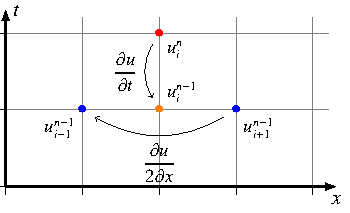
\includegraphics[width=.8\textwidth]{../tikz/linear3/linear3.pdf}
          \caption{linear Approach Derivative}
          \label{fig:STDL}
        \end{figure}

        \begin{figure}[!ht]
            \begin{minipage}[b]{0.5\textwidth}
              \includegraphics[width=1.1\textwidth]{../linear3_front.jpg}
              \caption{Linear Approach}
              \label{fig:STDL}
            \end{minipage}
            \begin{minipage}[b]{0.5\textwidth}
              \includegraphics[width=1\textwidth]{../linear3_top.jpg}
              \caption{Linear Approach}
              \label{fig:STDL}
            \end{minipage}
        \end{figure}
        \newpage

    \paragraph{Linear 4}

        \begin{equation}
            \frac{U_{t,x}-U_{t-1,x}}{\mathrm{dt}}+ U_{t,x}\, \frac{\left(U_{t-1,x+1}-U_{t-1,x-1}\right)}{2\mathrm{dx}}=0
        \end{equation}


        \begin{figure}[!ht]
          \centering
          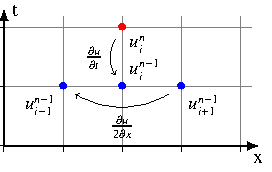
\includegraphics[width=.8\textwidth]{../tikz/linear4/linear4.pdf}
          \caption{linear Approach Derivative}
          \label{fig:STDL}
        \end{figure}

        \begin{figure}[!ht]
            \begin{minipage}[b]{0.5\textwidth}
              \includegraphics[width=1.1\textwidth]{../linear4_front.jpg}
              \caption{Linear Approach}
              \label{fig:STDL}
            \end{minipage}
            \begin{minipage}[b]{0.5\textwidth}
              \includegraphics[width=1\textwidth]{../linear4_top.jpg}
              \caption{Linear Approach}
              \label{fig:STDL}
            \end{minipage}
        \end{figure}


        \paragraph{Linear 5}



        \begin{equation}
          \frac{U-U_{t}}{\mathrm{dt}}+\frac{U_{t}\,\left(U-U_{x}\right)}{\mathrm{dx}}=0
        \end{equation}


        \begin{equation}
        U =  \frac{U_{t}\,\mathrm{dx}+U_{t}\,U_{x}\,\mathrm{dt}}{\mathrm{dx}+U_{t}\,\mathrm{dt}}
        \end{equation}

\end{document}
